\documentclass[tikz,border=9pt]{standalone}
\usepackage{amsmath}
\usetikzlibrary{arrows.meta}
\definecolor{practicegreen}{HTML}{245D34}
\definecolor{practiceink}{HTML}{222A24}
\begin{document}
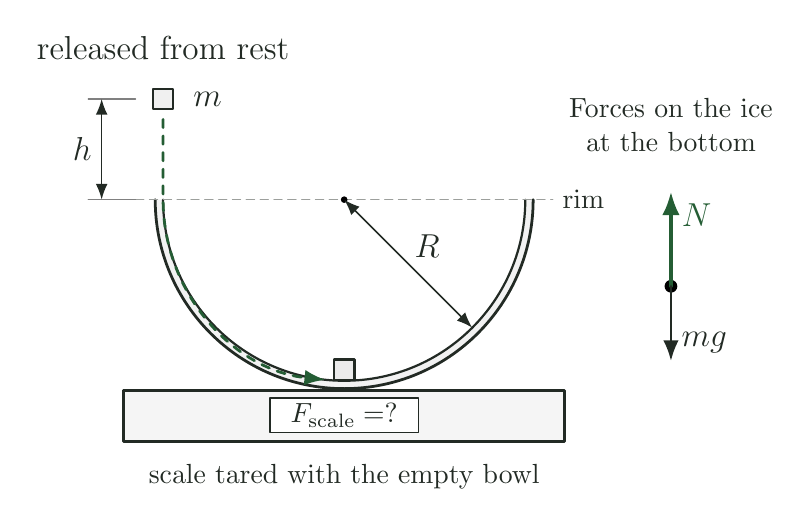
\begin{tikzpicture}[x=1cm,y=1cm,>=Latex,line cap=round,line join=round,
  draw=practiceink,text=practiceink,font=\large]
  % Hemispherical bowl: the rim lies at y=0; the bottom is a radius below it.
  \fill[black!5] (-2.4,0) arc[start angle=180,end angle=360,radius=2.4]
    --(2.3,0) arc[start angle=0,end angle=-180,radius=2.3] --cycle;
  \draw[line width=1pt] (-2.4,0) arc[start angle=180,end angle=360,radius=2.4];
  \draw[line width=.8pt] (-2.3,0) arc[start angle=180,end angle=360,radius=2.3];
  \draw[densely dashed,draw=practiceink!45] (-2.65,0)--(2.65,0) node[right,font=\normalsize]{rim};
  \fill (0,0) circle[radius=1.2pt];
  \draw[<->,line width=.6pt] (0,0)--(1.626,-1.626)
    node[midway,above right,fill=white,inner sep=2pt]{$R$};
  % Release and smooth path. The path is conceptual; the ice is a point mass.
  \draw[fill=black!6,line width=.8pt] (-2.43,1.15) rectangle (-2.17,1.41);
  \node[above] at (-2.3,1.65) {released from rest};
  \node[right] at (-2.04,1.28) {$m$};
  \draw[practicegreen,dashed,line width=1pt,->] (-2.3,1.02)--(-2.3,0)
    arc[start angle=180,end angle=264,radius=2.3];
  \draw[black!50,line width=.5pt] (-2.65,1.28)--(-3.25,1.28);
  \draw[black!50,line width=.5pt] (-2.65,0)--(-3.25,0);
  \draw[<->,line width=.6pt] (-3.08,0)--(-3.08,1.28) node[midway,left]{$h$};
  \draw[fill=black!8,line width=.8pt] (-.13,-2.29) rectangle (.13,-2.03);
  % Scale supports the bowl directly. Its empty-bowl reading is subtracted.
  \draw[line width=1pt,fill=black!4] (-2.8,-2.42) rectangle (2.8,-3.07);
  \draw[fill=white,line width=.5pt] (-.94,-2.52) rectangle (.94,-2.96);
  \node[font=\normalsize] at (0,-2.74) {$F_{\rm scale}=?$};
  \node[below,font=\normalsize] at (0,-3.24) {scale tared with the empty bowl};
  % Separate free-body diagram keeps forces from obscuring the bowl geometry.
  \node[font=\normalsize,align=center] at (4.15,.95) {Forces on the ice\\at the bottom};
  \fill (4.15,-1.1) circle[radius=2.3pt];
  \draw[->,practicegreen,line width=1.2pt] (4.15,-1.1)--(4.15,.1)
    node[right,near end]{$N$};
  \draw[->,line width=1pt] (4.15,-1.1)--(4.15,-2.05)
    node[right,near end]{$mg$};
\end{tikzpicture}
\end{document}
